% !TeX spellcheck = es_VE
% !TeX root = Informe.tex
%
% ESTADO: practica ejecutada el viernes 09/10/2026.
% Cubierto con evidencia: guia seccion 4 completa (sistema, NTP, Docker, contenedores
% de Prometheus y Grafana) y actividades 5.1 y 5.2.
% Fuera del informe por decision del equipo: actividad 5.3 y actividad 5.4.
%
% !TeX spellcheck = es_VE
\documentclass[12pt,letterpaper]{article}
\usepackage[utf8]{inputenc}
\usepackage{amsmath}
\usepackage{amsfonts}
\usepackage{amssymb}
\usepackage{graphicx}
\usepackage{url}
\usepackage{tikz}
\usepackage[shortlabels]{enumitem} % Se mantiene aquí con sus opciones
\usepackage{fancyhdr}
\usepackage[spanish]{babel}
%\usepackage[acronym]{glossaries}
%\makeglossaries

% agregar circuitos electronicos
\usepackage[siunitx, american]{circuitikz}

% comas sencillas en listing
\usepackage{textcomp}
\usepackage{upquote}
\usepackage{listings}
\lstset{upquote=true}

% dimensiones de pagina
\usepackage[left=1.5cm,top=1.5cm,right=1.5cm,bottom=2.5cm]{geometry}

% hiperenlaces
\usepackage{hyperref} % Para incluir hipervínculos
\hypersetup{urlcolor=blue,colorlinks=false,pdfborder={0 0 0}} % eliminar marco rojo en enlaces (citas, indices, pies de pagina, etc)

% permitir en la numeracion de los items agregar el numero de seccion
% (Se eliminó la línea duplicada \usepackage{enumitem} que causaba el error)
\setlist[enumerate]{label=\thesection.\arabic*. }   % numerar solo con seccion
%\setlist[enumerate]{label=\thesubsection.\arabic*. } % incluir numeracion de subsection

% otras configuraciones
\usepackage{parskip}
\setlength{\parskip}{1em} % establece el espacio entre parrafos
\setlength{\parindent}{0cm} % elimina la sangria inicial en parrafo
\usepackage{array} % ajustes adicionales para tablas
% \usepackage{pdfpages} %incluir archivos pdf en documento

% personalizacion de etiquetas
\renewcommand{\figurename}{Figura}
\renewcommand{\contentsname}{Contenido}
\renewcommand{\listfigurename}{Índice de Figuras}
\renewcommand{\listtablename}{Índice de Tablas}
\renewcommand{\lstlistlistingname}{Índice de Códigos}
\renewcommand{\tablename}{Tabla}
\renewcommand{\lstlistingname}{Código}

% pie de pagina
\renewcommand{\footrulewidth}{0.4pt}% grosor de linea del pie de pag
%\lfoot{\thepage} % texto izquierda
%\rfoot{\thepage} % texto derecha
\cfoot{\thepage} % texto al centro

%% definiciones para insertar codigo de programacion al doc
\usepackage{color}
\definecolor{dkgreen}{rgb}{0,0.6,0}
\definecolor{gray}{rgb}{0.5,0.5,0.5}
\definecolor{mauve}{rgb}{0.58,0,0.82}
\lstset{frame=tb,
    language=Python,
    aboveskip=3mm,
    belowskip=3mm,
    showstringspaces=false,
    columns=flexible,
    basicstyle={\small\ttfamily},
    %numbers=left,
    numberstyle=\tiny\color{gray},
    keywordstyle=\color{blue},
    commentstyle=\color{dkgreen},
    stringstyle=\color{mauve},
    breaklines=true,
    breakatwhitespace=true,
    tabsize=3
} % fin de codigo de programacion

%%%%%%%%%%%%%% MACRO PARA CONTROL DE PUNTAJE %%%%%%%%%%%%%%%%%%
\usepackage{xifthen}
\newcounter{puntos}
\setcounter{puntos}{0} % Inicializa el contador a cero

\newcommand{\sumarPunto}[1]{%
    \addtocounter{puntos}{#1}%
    \ifthenelse{#1 > 1}{(\textbf{#1 puntos})}{(\textbf{#1 punto})} 
}
%%%%%%%%%%%%%%%%%%%%%%%%%%%%%%%%%%%%%%%%%%%%%%%%%%%%%%%%%%
\usepackage[T1]{fontenc}

%%%%%%%%%%%%%%%%%%%%%%%%%%%%%%%%%%%%%%%%%%%%%%%%%%%%%%%%%%%%%%%%%%%%%%%
\pagestyle{fancy}
\fancyhf{}

\setlength{\headheight}{80pt}
\addtolength{\topmargin}{-35pt}
\setlength{\headsep}{1cm}
\setlength{\footskip}{20pt}

\rhead{
\includegraphics[width=1.3cm]{../img/logo_ciencias.png}}
\lhead{
\includegraphics[width=1.4cm]{../img/logo_ucv.png}}
\cfoot{\thepage}
\rfoot{Octubre, 2026}

\chead{Laboratorio de Internet de las Cosas}
\newcommand{\titulo}{LABORATORIO 6}
\newcommand{\subtitulo}{Visualización de datos con Grafana}
\newcommand{\autorUno}{Luisdavid Colina V24766381}
\newcommand{\autorDos}{Samantha Ramírez V31307714}

% Marca de trabajo pendiente, se elimina al cerrar el informe
\newcommand{\pendiente}[1]{%
  \par\vspace{0.3em}%
  \fbox{\parbox{0.97\linewidth}{\small\textit{Pendiente de ejecución en el
  laboratorio. #1}}}%
  \par\vspace{0.3em}%
}
%%%%%%%%%%%%%%%%%%%%%%%%%%%%%%%%%%%%%%%%%%%%%%%%%%%%%%%%%%%%%%%%%%%%%%%
\begin{document}

%%%%%%%%%%%%%%%%%%%%%%%%%%%%%%%%%%%%%%%%%%%%%%%%%%%%%%%%%%%%%%%%%%%%%%%
\begin{center}
  {\Large \textbf{\titulo}} \\[0.3cm]
  {\large \textbf{\subtitulo}} \\[0.8cm]

  \small
  \begin{tabular}{c}
    \textbf{Preparado por:} \\
    \autorUno \\
    \autorDos \\
  \end{tabular}
  \\[1cm]
\end{center}

%%%%%%%%%%%%%%%%%%%%%%%%%%%%%%%%%%%%%%%%%%%%%%%%%%%%%%%%%%%%%%%%%%%%%%%
\section{Equipo y herramientas}

El laboratorio anterior dejó un broker Mosquitto funcionando y la comprobación de
que los mensajes llegaban de una máquina a otra. Lo que faltaba era ver esos datos.
Una línea de texto en una terminal bastaría para confirmar que el enlace funciona, pero
no deja ver una tendencia ni comparar dos momentos. Grafana resuelve esa parte
leyendo de una fuente de datos y dibujando la serie en el tiempo~\cite{grafanadocs}.

La guía plantea el montaje sobre una Raspberry Pi con un sensor de ultrasonido
conectado a sus pines GPIO. El laboratorio no tenía Raspberry Pi disponible el día de
la práctica, así que el sensor se montó sobre una placa ESP32 con su tarjeta de
expansión, y toda la parte de servidor quedó en el PC de la mesa con Linux Mint. 

%%%%%%%%%%%%%%%%%%%%%%%%%%%%%%%%%%%%%%%%%%%%%%%%%%%%%%%%%%%%%%%%%%%%%%%
\section{Instalación del entorno}

%%%%%%%%%%%%%%%%%%%%%%%%%%%%%%%%%%%%%%%%%%%%%%%%%%%%%%%%%%%%%%%%%%%%%%%
\subsection{Actualización del sistema y servicio de tiempo}

El primer paso fue actualizar los paquetes e instalar \texttt{ntpsec}. Grafana ubica cada punto de la serie
según la marca de tiempo con la que llega, de modo que un reloj desfasado en el
equipo desplaza la gráfica completa y hace imposible comparar lo que publican dos
máquinas distintas.

\begin{lstlisting}[language=bash,
    caption={Actualización del sistema e instalación del servicio de tiempo.},
    label={lst:ntp},
    float=ht!]
sudo apt update && sudo apt upgrade -y
sudo apt-get install -y ntpsec
sudo systemctl status ntpsec --no-pager
\end{lstlisting}

El servicio quedó activo y sincronizando contra el grupo de servidores públicos
(Figura~\ref{fig:ntp_activo}).

\begin{figure}[ht!]
    \centering
    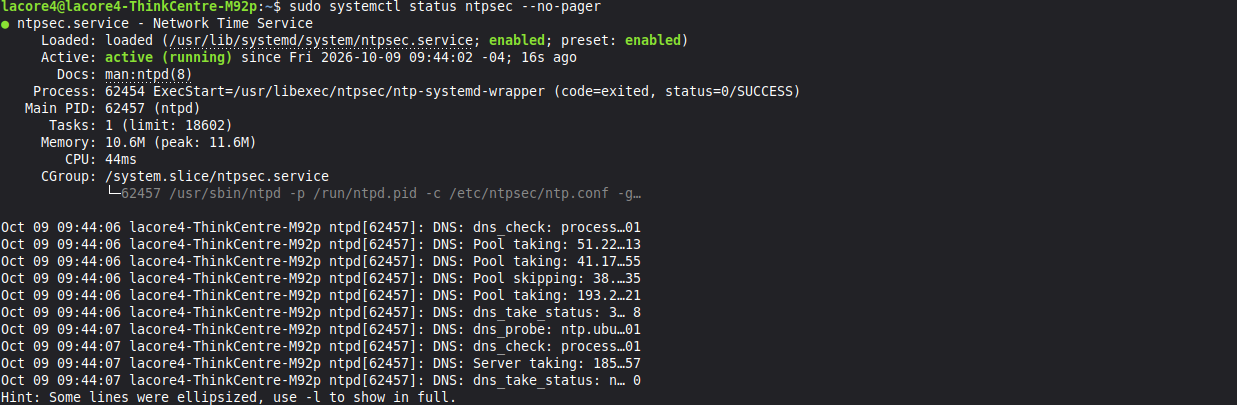
\includegraphics[width=\linewidth]{img/ntp_activo.png}
    \caption{Servicio \texttt{ntpsec} activo y resolviendo los servidores de tiempo.}
    \label{fig:ntp_activo}
\end{figure}

\pagebreak

%%%%%%%%%%%%%%%%%%%%%%%%%%%%%%%%%%%%%%%%%%%%%%%%%%%%%%%%%%%%%%%%%%%%%%%
\subsection{Docker y Docker Compose}

Grafana y Prometheus se instalaron como contenedores en lugar de paquetes del
sistema. La diferencia práctica es que la imagen trae sus propias dependencias y
versiones, así que no hay que pelear con las que ya tiene Linux Mint, y basta borrar
el contenedor para dejar el equipo como estaba.

La instalación siguió el repositorio oficial de Docker para Debian. Después de
instalar el motor se agregó el usuario al grupo \texttt{docker} y se ajustó el
permiso sobre el socket, que es lo que permite lanzar contenedores sin anteponer
\texttt{sudo} a cada comando. Las versiones que quedaron instaladas se ven en la
Figura~\ref{fig:docker_version}.

\begin{lstlisting}[language=bash,
    caption={Permiso de acceso al socket de Docker.},
    label={lst:setfacl},
    float=ht!]
sudo usermod -aG docker $USER
sudo setfacl -m user:$USER:rw /var/run/docker.sock
\end{lstlisting}

\begin{figure}[ht!]
    \centering
    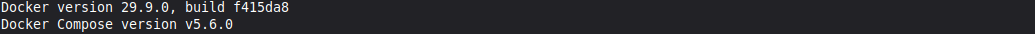
\includegraphics[width=0.85\linewidth]{img/docker_version.png}
    \caption{Versiones instaladas del motor y del complemento Compose.}
    \label{fig:docker_version}
\end{figure}

%%%%%%%%%%%%%%%%%%%%%%%%%%%%%%%%%%%%%%%%%%%%%%%%%%%%%%%%%%%%%%%%%%%%%%%
\subsection{Contenedores de Prometheus y Grafana}

Con el motor listo se creó el directorio \texttt{contenedor} con los tres archivos de
configuración que pide la guía. El \texttt{docker-compose.yml} declara los dos
servicios, publica el puerto 9090 para Prometheus y el 3000 para Grafana, y enlaza el
segundo con el primero. Los \textit{paths} de los volúmenes van absolutos, tal como
advierte el enunciado, porque Compose interpreta cualquier ruta relativa como el
nombre de un volumen con nombre y no como una carpeta del disco.

\begin{lstlisting}[language=bash,
    caption={Archivos de configuración y arranque de los contenedores.},
    label={lst:compose},
    float=ht!]
mkdir -p /home/$USER/contenedor
cd /home/$USER/contenedor
nano docker-compose.yml
nano prometheus.yml
touch grafana.yml
chmod 755 *
docker compose up -d
\end{lstlisting}

La descarga de las dos imágenes tomó un minuto y medio, y los
contenedores quedaron levantados a la primera (Figura~\ref{fig:contenedores}).
Prometheus se instaló aunque no se usó en el laboratorio.

\begin{figure}[ht!]
    \centering
    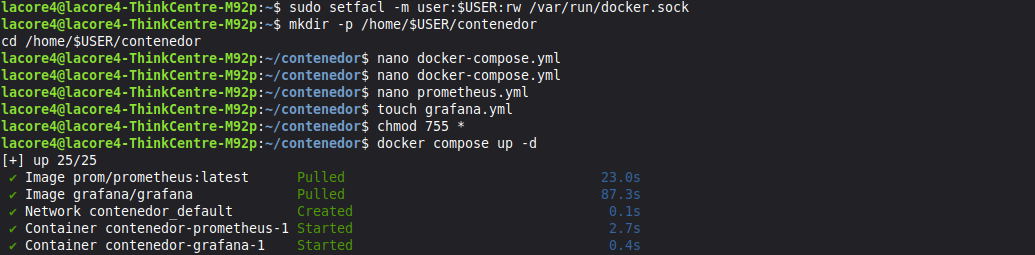
\includegraphics[width=\linewidth]{img/contenedores_arriba.png}
    \caption{Creación de los archivos y arranque de los dos contenedores.}
    \label{fig:contenedores}
\end{figure}

\pagebreak

Ambas interfaces respondieron desde el navegador del mismo equipo. Prometheus quedó
en el puerto 9090 con su consola de consultas vacía
(Figura~\ref{fig:prometheus}), y Grafana en el 3000, donde el primer acceso pide
cambiar la contraseña \texttt{admin} que trae por defecto.

\begin{figure}[ht!]
    \centering
    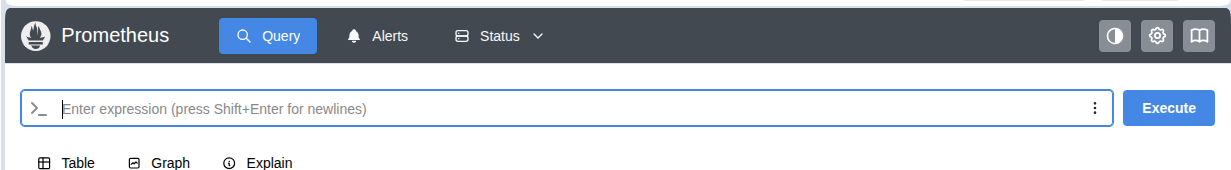
\includegraphics[width=\linewidth]{img/prometheus_interfaz.png}
    \caption{Consola de consultas de Prometheus en el puerto 9090.}
    \label{fig:prometheus}
\end{figure}

\clearpage
%%%%%%%%%%%%%%%%%%%%%%%%%%%%%%%%%%%%%%%%%%%%%%%%%%%%%%%%%%%%%%%%%%%%%%%
\section{Adquisición de datos del sensor}

%%%%%%%%%%%%%%%%%%%%%%%%%%%%%%%%%%%%%%%%%%%%%%%%%%%%%%%%%%%%%%%%%%%%%%%
\subsection{Conexión del sensor y script de recepción}
\textit{Enunciado: Conecte el sensor de Ultrasonidos a la placa. Programe un script en
Python que sea capaz de recibir los datos enviados por el sensor. Muestre el circuito
en Fritzing. (5 puntos)}

El montaje se hizo sobre hardware real y no en Fritzing, el circuito se ve en la (Figura~\ref{fig:montaje_sensor}). El HC-SR04
tiene cuatro terminales. \texttt{VCC} y \texttt{GND} toman la alimentación de los
rieles de la protoboard, \texttt{TRIG} recibe el pulso que dispara la medición y
\texttt{ECHO} devuelve un pulso cuya duración es proporcional al tiempo de vuelo del
sonido~\cite{hcsr04}.

\begin{center}
\small
\begin{tabular}{ll}
\hline
\textbf{Terminal del sensor} & \textbf{Conexión en la placa} \\
\hline
\texttt{VCC}  & Riel de alimentación de la protoboard \\
\texttt{GND}  & Riel de tierra de la protoboard \\
\texttt{TRIG} & GPIO 12, configurado como salida \\
\texttt{ECHO} & GPIO 14, configurado como entrada \\
\hline
\end{tabular}
\end{center}

\begin{figure}[ht!]
    \centering
    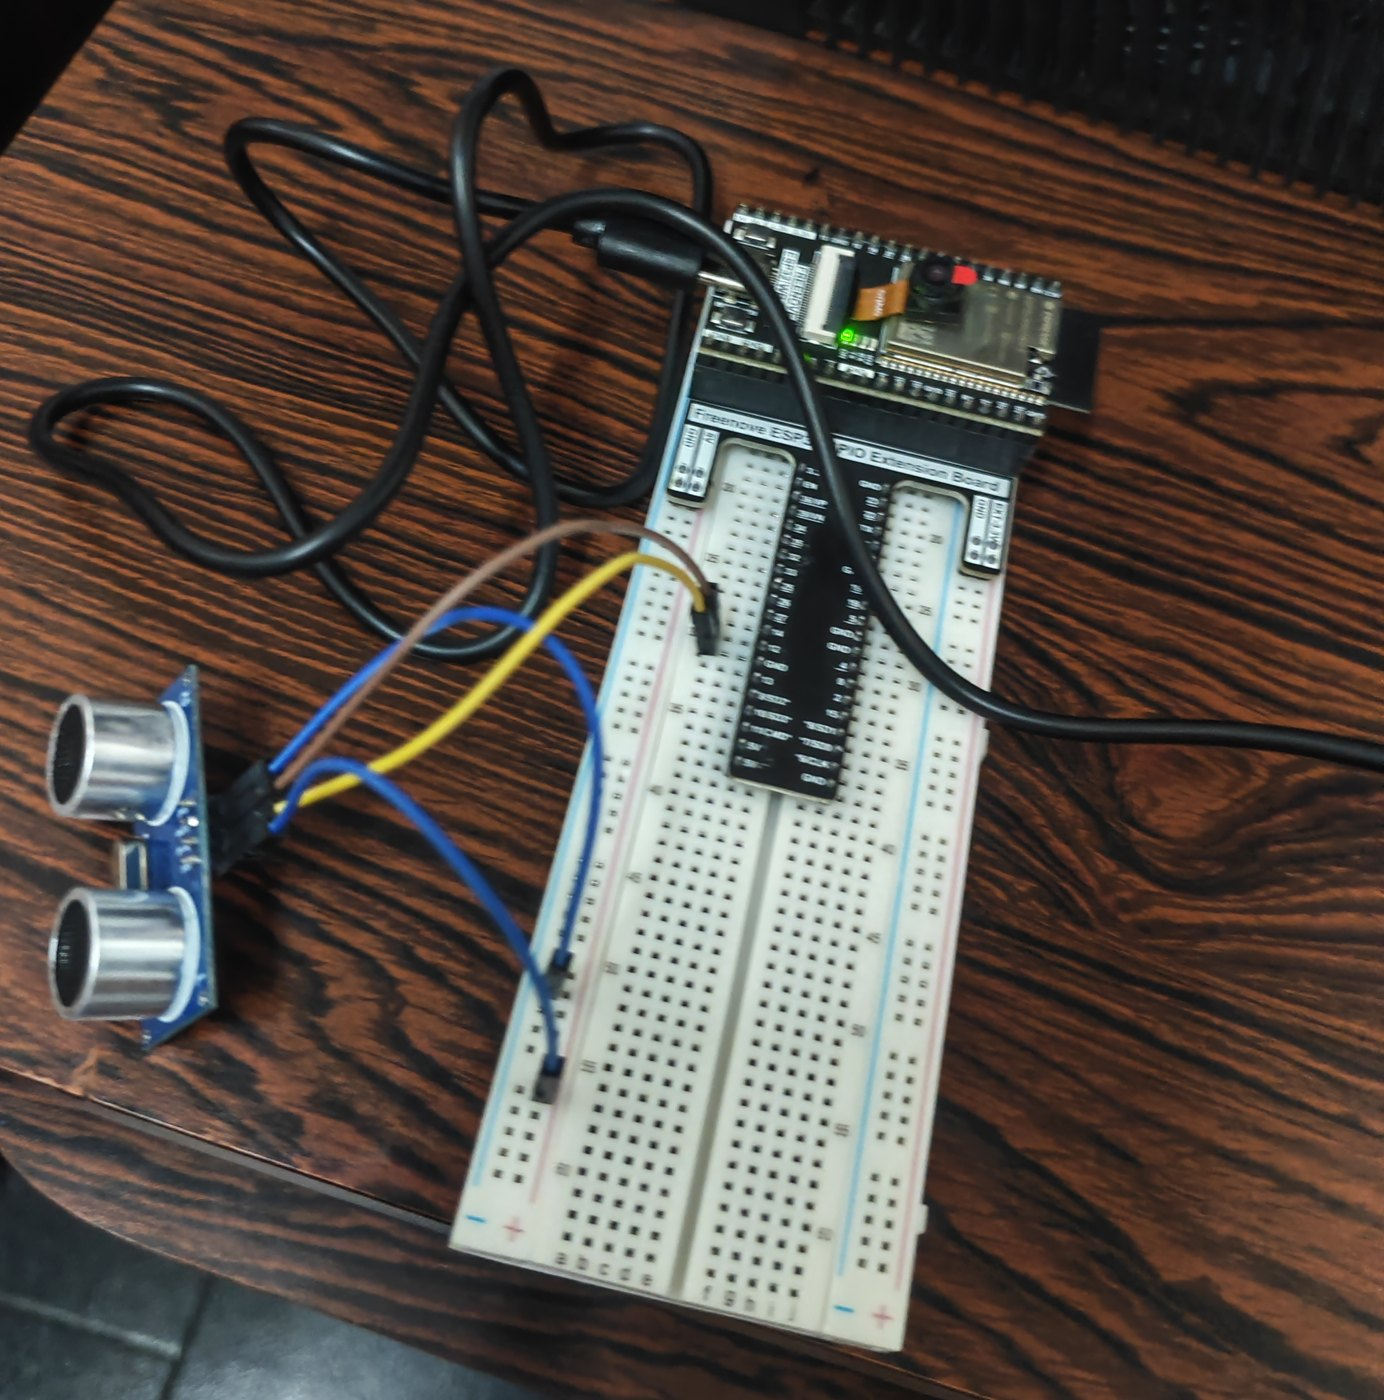
\includegraphics[width=0.62\linewidth]{img/montaje_sensor.jpg}
    \caption{Montaje del HC-SR04 sobre la protoboard junto a la placa ESP32.}
    \label{fig:montaje_sensor}
\end{figure}

\pagebreak

\textbf{Firmware de la placa.} La placa venía sin MicroPython, así que primero hubo
que grabarlo. El trabajo se hizo desde un entorno virtual de Python con
\texttt{esptool} para borrar y escribir la memoria flash, y \texttt{mpremote} para
copiar archivos a la placa ya encendida~\cite{micropython}. La secuencia completa
quedó registrada en la Figura~\ref{fig:flasheo}.

\begin{figure}[ht!]
    \centering
    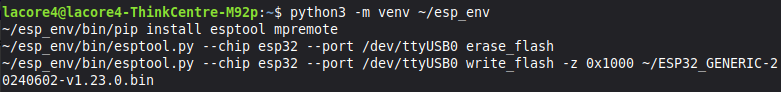
\includegraphics[width=\linewidth]{img/flasheo_esp32.png}
    \caption{Entorno virtual, herramientas y grabado del firmware MicroPython.}
    \label{fig:flasheo}
\end{figure}

El borrado previo con \texttt{erase\_flash} no es opcional. Sin él, los restos del
firmware anterior conviven con el nuevo en la misma memoria y la placa arranca en un
estado indefinido. La escritura terminó verificando el \textit{hash} de lo grabado y
reiniciando la placa por la línea RTS (Figura~\ref{fig:firmware}).

\begin{figure}[ht!]
    \centering
    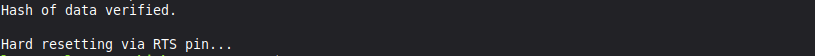
\includegraphics[width=0.85\linewidth]{img/firmware_verificado.png}
    \caption{Verificación del firmware grabado y reinicio de la placa.}
    \label{fig:firmware}
\end{figure}

El programa que corre en la placa, \texttt{main.py} en la
Figura~\ref{fig:main_py}, calcula la distancia a partir del tiempo de vuelo.
Pone \texttt{TRIG} en alto durante diez microsegundos, mide con
\texttt{time\_pulse\_us()} cuánto dura el pulso de \texttt{ECHO} y aplica la velocidad
del sonido, 343 metros por segundo, dividiendo entre dos porque el sonido recorre el
camino de ida y vuelta. El tercer argumento de \texttt{time\_pulse\_us()} es un tiempo
de espera de 30 milisegundos que evita que el programa se quede trabado cuando no hay
eco de retorno, caso en el que la función devuelve un valor negativo y la medición se
reporta como cero.

\begin{figure}[ht!]
    \centering
    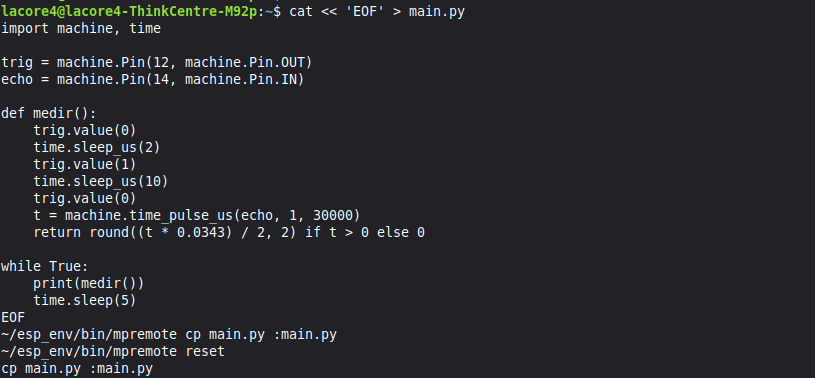
\includegraphics[width=0.85\linewidth]{img/main_py.png}
    \caption{Programa \texttt{main.py} escrito en la placa y copiado con
    \texttt{mpremote}.}
    \label{fig:main_py}
\end{figure}

El intervalo entre lecturas arrancó en cinco segundos, como se ve en esa misma figura, y
después se bajó a medio segundo. Con cinco segundos la gráfica de Grafana quedaba
con puntos demasiado separados y el trazo parecía una línea recta entre dos
mediciones lejanas.

\pagebreak

\textbf{Recepción desde Python.} Del lado del PC, la placa aparece como el archivo de
dispositivo \texttt{/dev/ttyUSB0}. El script abre ese puerto a 115200 baudios con
\texttt{pyserial} y lee línea por línea lo que la placa imprime~\cite{pyserial}. La
conversión a \texttt{float} dentro de un \texttt{try} es necesaria porque al conectar
la placa el puerto entrega además mensajes de arranque de MicroPython, que no son
números y harían fallar el programa.

%%%%%%%%%%%%%%%%%%%%%%%%%%%%%%%%%%%%%%%%%%%%%%%%%%%%%%%%%%%%%%%%%%%%%%%
\section{Publicación y visualización}

%%%%%%%%%%%%%%%%%%%%%%%%%%%%%%%%%%%%%%%%%%%%%%%%%%%%%%%%%%%%%%%%%%%%%%%
\subsection{Tópicos en el broker y panel en Grafana}
\textit{Enunciado: El script debe publicar los datos recibidos como tópicos y
enviarlos al broker mosquitto. Siga la siguiente nomenclatura para los tópicos
\texttt{/NombreGrupo/distancia}, \texttt{/NombreGrupo/temperatura},
\texttt{/NombreGrupo/humedad}. Visualice sus tópicos en Grafana. (5 puntos)}

\textbf{Prueba previa contra el broker.} Antes de conectar el sensor se corrió un
script que publicaba números aleatorios en los tres tópicos. Las distancias, las
temperaturas y las humedades de la Figura~\ref{fig:telemetria} no salen de ninguna
medición, las genera el propio script. El objetivo era comprobar que el cliente se
autenticaba contra Mosquitto y que los tópicos llegaban, de modo que cualquier falla
posterior tenía que venir de la placa o del puerto serial y no de la red.

\begin{figure}[ht!]
    \centering
    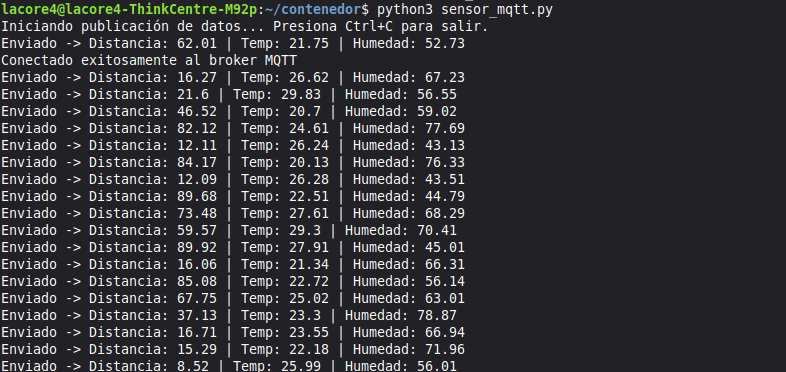
\includegraphics[width=0.85\linewidth]{img/telemetria_broker.png}
    \caption{Prueba del enlace con el broker usando números aleatorios, antes de
    conectar el sensor.}
    \label{fig:telemetria}
\end{figure}

\pagebreak

\textbf{Puente entre el puerto serial y el broker.} El programa definitivo junta las
dos mitades. Lee del puerto serial lo que escribe la placa y publica cada lectura en
\texttt{/Grupo1/distancia} con \texttt{paho-mqtt}~\cite{paho}.

Los otros dos tópicos de la nomenclatura llevan un valor fijo de 25,0 y 60,0. El
único sensor disponible en la mesa fue el de ultrasonido, que mide distancia y nada
más, así que no había de dónde sacar temperatura ni humedad reales. Los tópicos se
mantienen publicándose para respetar el esquema de nombres que pide el enunciado, y
quedan marcados como simulados en el propio código para que no se confundan con una
medición (Figura~\ref{fig:puente_py}).

\begin{figure}[ht!]
    \centering
    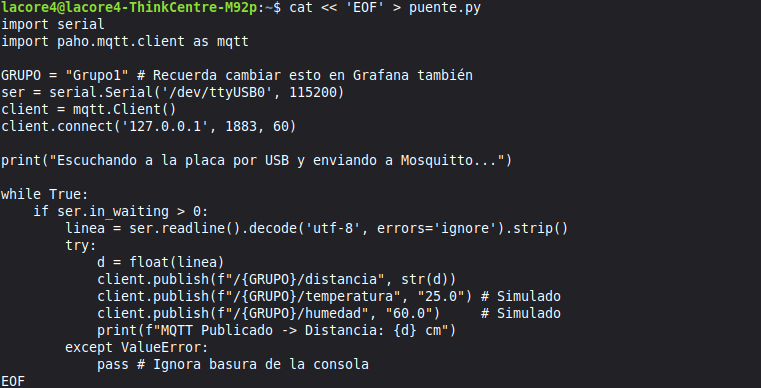
\includegraphics[width=0.95\linewidth]{img/puente_py.png}
    \caption{Programa \texttt{puente.py} que lee el puerto serial y publica al broker.}
    \label{fig:puente_py}
\end{figure}

El primer intento de ejecución falló porque \texttt{paho-mqtt} no estaba instalado en
el entorno virtual. El error es explícito y se resolvió con una instalación en el
mismo entorno, junto con \texttt{pyserial} (Figura~\ref{fig:paho}).

\begin{figure}[ht!]
    \centering
    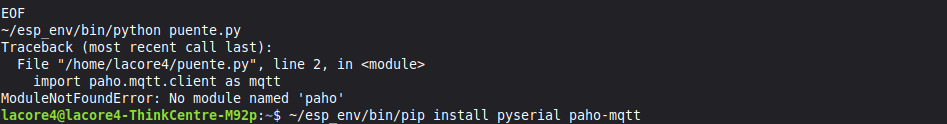
\includegraphics[width=0.95\linewidth]{img/dependencia_paho.png}
    \caption{Falta de la librería \texttt{paho} y su instalación en el entorno virtual.}
    \label{fig:paho}
\end{figure}

\pagebreak

Con la dependencia resuelta, el puente quedó publicando una medición cada medio
segundo (Figura~\ref{fig:publicacion}). La advertencia sobre la versión 1 de la API
de \textit{callbacks} que aparece al arrancar no interrumpe nada, solo avisa que
\texttt{mqtt.Client()} sin argumentos usa la interfaz anterior de la librería.

\begin{figure}[ht!]
    \centering
    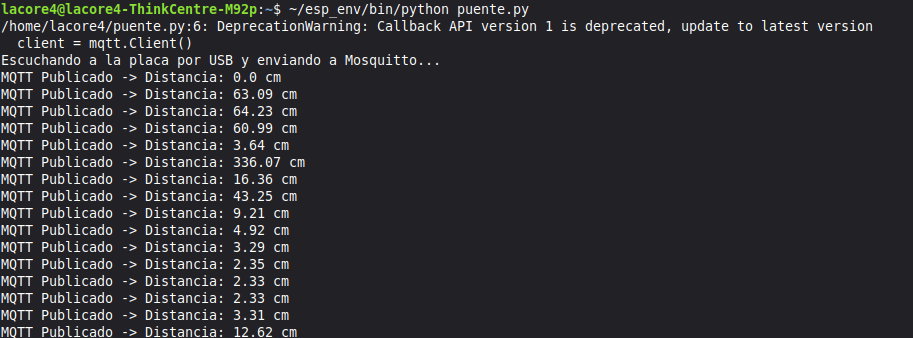
\includegraphics[width=0.95\linewidth]{img/publicacion_mqtt.png}
    \caption{Publicación continua de las lecturas del sensor hacia el broker.}
    \label{fig:publicacion}
\end{figure}

Las lecturas que salen por la terminal corresponden a objetos colocados a pocos
centímetros del sensor, como se aprecia en la Figura~\ref{fig:montaje_publicando}.

\begin{figure}[ht!]
    \centering
    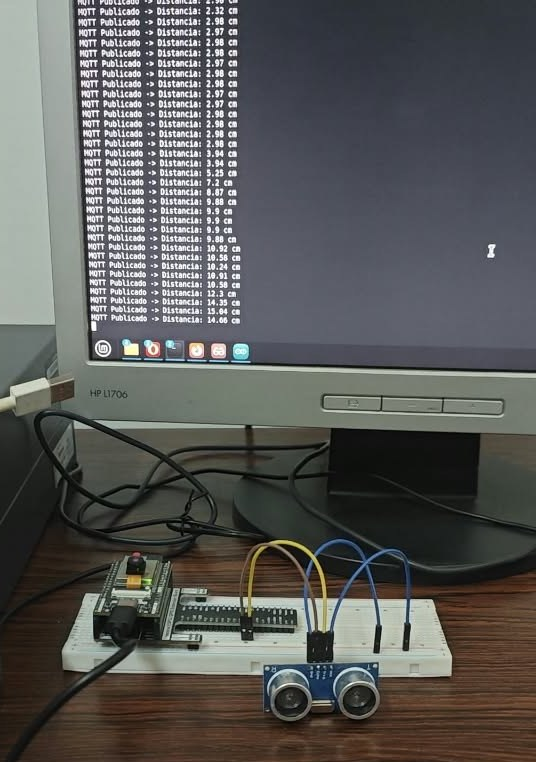
\includegraphics[width=0.40\linewidth]{img/montaje_publicando.jpg}
    \caption{Montaje publicando al broker, con la salida del puente en la pantalla.}
    \label{fig:montaje_publicando}
\end{figure}

\textbf{Visualización en Grafana.} En Grafana se agregó la fuente de datos MQTT
apuntando al broker local y se armó un panel sobre el tópico
\texttt{/Grupo1/distancia}~\cite{mqttdatasource}. La gráfica responde en vivo al
movimiento de un objeto frente al sensor
(Figura~\ref{fig:panel}). El valor señalado en el panel, 27,8 centímetros a las
10:14:26, corresponde a una de las lecturas publicadas por el puente.

\begin{figure}[ht!]
    \centering
    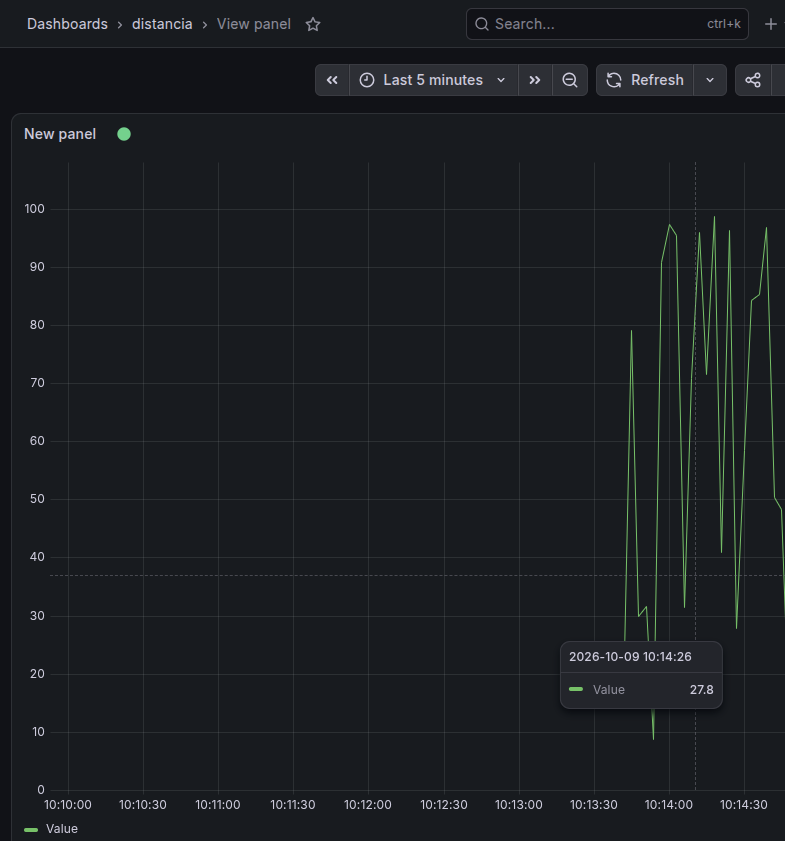
\includegraphics[width=0.46\linewidth]{img/panel_distancia.png}
    \caption{Panel de Grafana con la serie del tópico \texttt{/Grupo1/distancia}.}
    \label{fig:panel}
\end{figure}

Los valores altos aislados que se ven en la serie, por encima de los 300 centímetros,
no son un error del montaje. Ocurren cuando el pulso de ultrasonido no encuentra una
superficie perpendicular y rebota contra algo lejano antes de volver, de modo que el
tiempo de vuelo medido es mayor que el real. Con el objeto quieto frente al sensor la
serie se mantiene estable.

La relación entre lo que ocurre sobre la mesa y lo que dibuja el panel se ve mejor en
la Figura~\ref{fig:respuesta_sensor}. Los tramos planos de la serie corresponden al
objeto sostenido a una distancia fija, y los saltos a los momentos en que se acerca o
se aleja del sensor. La Figura~\ref{fig:montaje_grafana} muestra el mismo puesto de
trabajo visto de frente, con el panel actualizándose mientras el puente publica.

\begin{figure}[ht!]
    \centering
    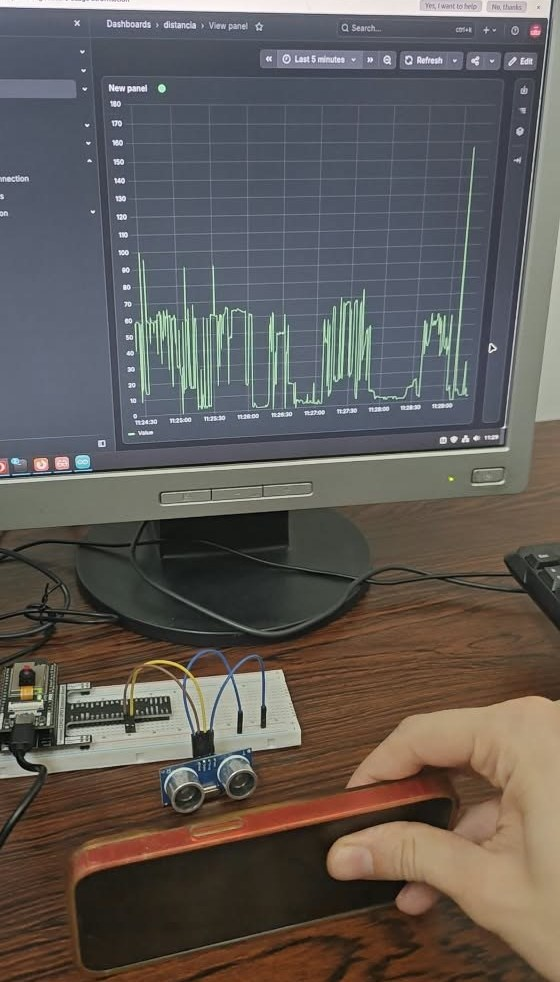
\includegraphics[width=0.40\linewidth]{img/respuesta_sensor.jpg}
    \caption{Respuesta del panel al acercar un objeto al sensor.}
    \label{fig:respuesta_sensor}
\end{figure}

\begin{figure}[ht!]
    \centering
    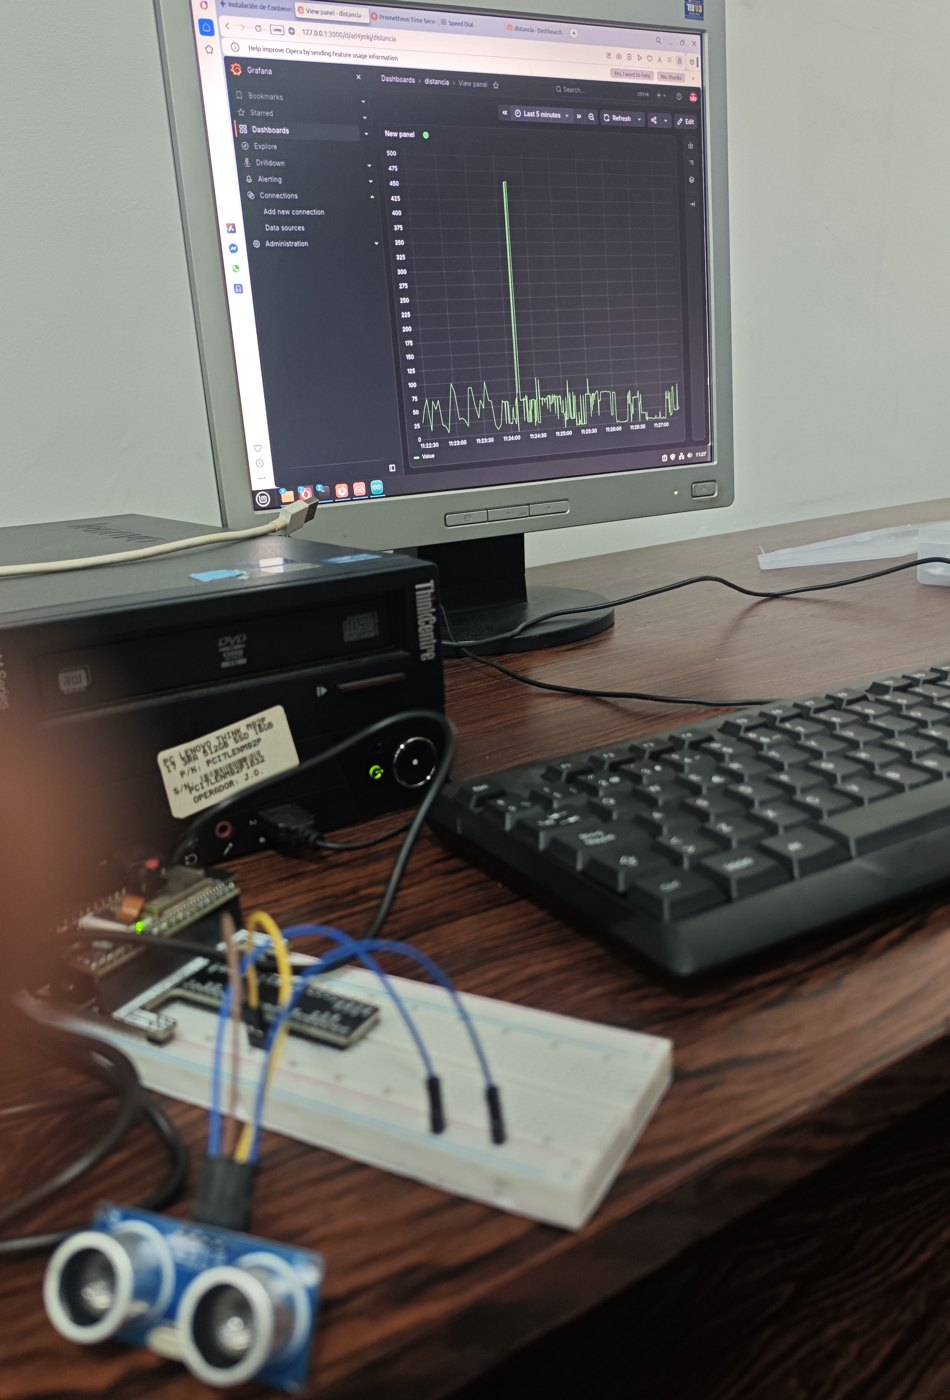
\includegraphics[width=0.26\linewidth]{img/montaje_grafana.jpg}
    \caption{Montaje en funcionamiento con el panel de Grafana actualizándose.}
    \label{fig:montaje_grafana}
\end{figure}

\clearpage
%%%%%%%%%%%%%%%%%%%%%%%%%%%%%%%%%%%%%%%%%%%%%%%%%%%%%%%%%%%%%%%%%%%%%%%
\section{Conclusiones}

El laboratorio cerró la cadena completa de un sistema IoT básico. El sensor entrega
una medición física, el microcontrolador la convierte en un número, un programa en el
PC la publica en el broker y Grafana la dibuja. Cada pieza habla con la siguiente por
un protocolo distinto, y ninguna necesita saber cómo funcionan las demás.

La pieza que hizo falta construir fue el puente. El ESP32 no habla MQTT por el cable
USB, solo escribe texto en el puerto serial, y Grafana no lee puertos seriales. Ese
programa de veinte líneas es el que traduce entre los dos mundos, y es también el
lugar donde se decide el nombre del tópico, que es lo que después permite distinguir
el dato de un grupo del de otro dentro del mismo broker.

Trabajar con contenedores cambió la forma de montar el servidor respecto a los
laboratorios anteriores. Mosquitto se instaló con \texttt{apt} y quedó mezclado con
el resto del sistema, mientras que Prometheus y Grafana se levantaron con un solo
comando y se pueden borrar sin dejar rastro. El precio es que los archivos de
configuración tienen que ir montados con rutas absolutas desde el disco, porque el
contenedor no ve el sistema de archivos del equipo.

El punto que más tiempo consumió no fue ninguno de los conceptos del laboratorio,
sino el grabado del firmware en la placa. La memoria flash hay que borrarla antes de
escribirla, la escritura toma cerca de dos minutos y el entorno virtual de Python
tiene que tener cada librería instalada dentro, no en el sistema. Son pasos
mecánicos, pero cualquiera que se salte deja la placa en un estado en el que no
responde y no hay un mensaje de error que apunte a la causa.

Queda clara también la utilidad de la visualización. Las mismas lecturas que en la
terminal son una lista de números sin forma, en la gráfica muestran de inmediato el
rango habitual de la medición y las mediciones sueltas que se salen de ese rango.

\clearpage
%%%%%%%%%%%%%%%%%%%%%%%%%%%%%%%%%%%%%%%%%%%%%%%%%%%%%%%%%%%%%%%%%%%%%%%
\begingroup
\small
\begin{thebibliography}{9}

\bibitem{grafanadocs}
Grafana Labs, ``Run Grafana Docker image,'' \emph{Grafana Documentation}, 2024.
[En línea]. Disponible:
\url{https://grafana.com/docs/grafana/latest/setup-grafana/installation/docker/}.
[Consulta: oct.~2026]

\bibitem{mqttdatasource}
Grafana Labs, ``MQTT data source for Grafana,'' \emph{GitHub Repository}, 2024.
[En línea]. Disponible: \url{https://github.com/grafana/mqtt-datasource}.
[Consulta: oct.~2026]

\bibitem{micropython}
MicroPython, ``Quick reference for the ESP32,'' \emph{MicroPython Documentation},
2024. [En línea]. Disponible:
\url{https://docs.micropython.org/en/latest/esp32/quickref.html}.
[Consulta: oct.~2026]

\bibitem{hcsr04}
Elec Freaks, ``Ultrasonic Ranging Module HC-SR04,'' hoja de datos técnica, 2024.
[En línea]. Disponible:
\url{https://cdn.sparkfun.com/datasheets/Sensors/Proximity/HCSR04.pdf}.
[Consulta: oct.~2026]

\bibitem{pyserial}
C.~Liechti, ``pySerial Documentation,'' 2001--2024. [En línea]. Disponible:
\url{https://pyserial.readthedocs.io/en/latest/}. [Consulta: oct.~2026]

\bibitem{paho}
Eclipse Foundation, ``Eclipse Paho MQTT Python Client,'' 2024. [En línea].
Disponible:
\url{https://eclipse.dev/paho/index.php?page=clients/python/index.php}.
[Consulta: oct.~2026]

\end{thebibliography}
\endgroup

\end{document}
